% Options for packages loaded elsewhere
\PassOptionsToPackage{unicode}{hyperref}
\PassOptionsToPackage{hyphens}{url}
%
\documentclass[
  man,mask]{apa7}
\usepackage{amsmath,amssymb}
\usepackage{iftex}
\ifPDFTeX
  \usepackage[T1]{fontenc}
  \usepackage[utf8]{inputenc}
  \usepackage{textcomp} % provide euro and other symbols
\else % if luatex or xetex
  \usepackage{unicode-math} % this also loads fontspec
  \defaultfontfeatures{Scale=MatchLowercase}
  \defaultfontfeatures[\rmfamily]{Ligatures=TeX,Scale=1}
\fi
\usepackage{lmodern}
\ifPDFTeX\else
  % xetex/luatex font selection
\fi
% Use upquote if available, for straight quotes in verbatim environments
\IfFileExists{upquote.sty}{\usepackage{upquote}}{}
\IfFileExists{microtype.sty}{% use microtype if available
  \usepackage[]{microtype}
  \UseMicrotypeSet[protrusion]{basicmath} % disable protrusion for tt fonts
}{}
\makeatletter
\@ifundefined{KOMAClassName}{% if non-KOMA class
  \IfFileExists{parskip.sty}{%
    \usepackage{parskip}
  }{% else
    \setlength{\parindent}{0pt}
    \setlength{\parskip}{6pt plus 2pt minus 1pt}}
}{% if KOMA class
  \KOMAoptions{parskip=half}}
\makeatother
\usepackage{xcolor}
\usepackage{graphicx}
\makeatletter
\def\maxwidth{\ifdim\Gin@nat@width>\linewidth\linewidth\else\Gin@nat@width\fi}
\def\maxheight{\ifdim\Gin@nat@height>\textheight\textheight\else\Gin@nat@height\fi}
\makeatother
% Scale images if necessary, so that they will not overflow the page
% margins by default, and it is still possible to overwrite the defaults
% using explicit options in \includegraphics[width, height, ...]{}
\setkeys{Gin}{width=\maxwidth,height=\maxheight,keepaspectratio}
% Set default figure placement to htbp
\makeatletter
\def\fps@figure{htbp}
\makeatother
\setlength{\emergencystretch}{3em} % prevent overfull lines
\providecommand{\tightlist}{%
  \setlength{\itemsep}{0pt}\setlength{\parskip}{0pt}}
\setcounter{secnumdepth}{-\maxdimen} % remove section numbering
% Make \paragraph and \subparagraph free-standing
\ifx\paragraph\undefined\else
  \let\oldparagraph\paragraph
  \renewcommand{\paragraph}[1]{\oldparagraph{#1}\mbox{}}
\fi
\ifx\subparagraph\undefined\else
  \let\oldsubparagraph\subparagraph
  \renewcommand{\subparagraph}[1]{\oldsubparagraph{#1}\mbox{}}
\fi
% definitions for citeproc citations
\NewDocumentCommand\citeproctext{}{}
\NewDocumentCommand\citeproc{mm}{%
  \begingroup\def\citeproctext{#2}\cite{#1}\endgroup}
\makeatletter
 % allow citations to break across lines
 \let\@cite@ofmt\@firstofone
 % avoid brackets around text for \cite:
 \def\@biblabel#1{}
 \def\@cite#1#2{{#1\if@tempswa , #2\fi}}
\makeatother
\newlength{\cslhangindent}
\setlength{\cslhangindent}{1.5em}
\newlength{\csllabelwidth}
\setlength{\csllabelwidth}{3em}
\newenvironment{CSLReferences}[2] % #1 hanging-indent, #2 entry-spacing
 {\begin{list}{}{%
  \setlength{\itemindent}{0pt}
  \setlength{\leftmargin}{0pt}
  \setlength{\parsep}{0pt}
  % turn on hanging indent if param 1 is 1
  \ifodd #1
   \setlength{\leftmargin}{\cslhangindent}
   \setlength{\itemindent}{-1\cslhangindent}
  \fi
  % set entry spacing
  \setlength{\itemsep}{#2\baselineskip}}}
 {\end{list}}
\usepackage{calc}
\newcommand{\CSLBlock}[1]{\hfill\break\parbox[t]{\linewidth}{\strut\ignorespaces#1\strut}}
\newcommand{\CSLLeftMargin}[1]{\parbox[t]{\csllabelwidth}{\strut#1\strut}}
\newcommand{\CSLRightInline}[1]{\parbox[t]{\linewidth - \csllabelwidth}{\strut#1\strut}}
\newcommand{\CSLIndent}[1]{\hspace{\cslhangindent}#1}
\ifLuaTeX
\usepackage[bidi=basic]{babel}
\else
\usepackage[bidi=default]{babel}
\fi
\babelprovide[main,import]{english}
% get rid of language-specific shorthands (see #6817):
\let\LanguageShortHands\languageshorthands
\def\languageshorthands#1{}
% Manuscript styling
\usepackage{upgreek}
\captionsetup{font=singlespacing,justification=justified}

% Table formatting
\usepackage{longtable}
\usepackage{lscape}
% \usepackage[counterclockwise]{rotating}   % Landscape page setup for large tables
\usepackage{multirow}		% Table styling
\usepackage{tabularx}		% Control Column width
\usepackage[flushleft]{threeparttable}	% Allows for three part tables with a specified notes section
\usepackage{threeparttablex}            % Lets threeparttable work with longtable

% Create new environments so endfloat can handle them
% \newenvironment{ltable}
%   {\begin{landscape}\centering\begin{threeparttable}}
%   {\end{threeparttable}\end{landscape}}
\newenvironment{lltable}{\begin{landscape}\centering\begin{ThreePartTable}}{\end{ThreePartTable}\end{landscape}}

% Enables adjusting longtable caption width to table width
% Solution found at http://golatex.de/longtable-mit-caption-so-breit-wie-die-tabelle-t15767.html
\makeatletter
\newcommand\LastLTentrywidth{1em}
\newlength\longtablewidth
\setlength{\longtablewidth}{1in}
\newcommand{\getlongtablewidth}{\begingroup \ifcsname LT@\roman{LT@tables}\endcsname \global\longtablewidth=0pt \renewcommand{\LT@entry}[2]{\global\advance\longtablewidth by ##2\relax\gdef\LastLTentrywidth{##2}}\@nameuse{LT@\roman{LT@tables}} \fi \endgroup}

% \setlength{\parindent}{0.5in}
% \setlength{\parskip}{0pt plus 0pt minus 0pt}

% Overwrite redefinition of paragraph and subparagraph by the default LaTeX template
% See https://github.com/crsh/papaja/issues/292
\makeatletter
\renewcommand{\paragraph}{\@startsection{paragraph}{4}{\parindent}%
  {0\baselineskip \@plus 0.2ex \@minus 0.2ex}%
  {-1em}%
  {\normalfont\normalsize\bfseries\itshape\typesectitle}}

\renewcommand{\subparagraph}[1]{\@startsection{subparagraph}{5}{1em}%
  {0\baselineskip \@plus 0.2ex \@minus 0.2ex}%
  {-\z@\relax}%
  {\normalfont\normalsize\itshape\hspace{\parindent}{#1}\textit{\addperi}}{\relax}}
\makeatother

\makeatletter
\usepackage{etoolbox}
\patchcmd{\maketitle}
  {\section{\normalfont\normalsize\abstractname}}
  {\section*{\normalfont\normalsize\abstractname}}
  {}{\typeout{Failed to patch abstract.}}
\patchcmd{\maketitle}
  {\section{\protect\normalfont{\@title}}}
  {\section*{\protect\normalfont{\@title}}}
  {}{\typeout{Failed to patch title.}}
\makeatother

\usepackage{xpatch}
\makeatletter
\xapptocmd\appendix
  {\xapptocmd\section
    {\addcontentsline{toc}{section}{\appendixname\ifoneappendix\else~\theappendix\fi\\: #1}}
    {}{\InnerPatchFailed}%
  }
{}{\PatchFailed}
\keywords{Survey methodology, sample weighting, nonresponse, response rate}
\DeclareDelayedFloatFlavor{ThreePartTable}{table}
\DeclareDelayedFloatFlavor{lltable}{table}
\DeclareDelayedFloatFlavor*{longtable}{table}
\makeatletter
\renewcommand{\efloat@iwrite}[1]{\immediate\expandafter\protected@write\csname efloat@post#1\endcsname{}}
\makeatother
\usepackage{lineno}

\linenumbers
\usepackage{csquotes}
\raggedbottom
\ifLuaTeX
  \usepackage{selnolig}  % disable illegal ligatures
\fi
\usepackage{bookmark}
\IfFileExists{xurl.sty}{\usepackage{xurl}}{} % add URL line breaks if available
\urlstyle{same}
\hypersetup{
  pdftitle={Nonresponse and Sample Weighting in Organizational Surveying},
  pdflang={en-EN},
  pdfkeywords={Survey methodology, sample weighting, nonresponse, response rate},
  hidelinks,
  pdfcreator={LaTeX via pandoc}}

\title{Nonresponse and Sample Weighting in Organizational Surveying}
\author{John T. Kulas\textsuperscript{1}, Yang Yang\textsuperscript{2}, \& David H. Robinson\textsuperscript{3}}
\date{}


\shorttitle{NONRESPONSE AND SAMPLE WEIGHTING}

\authornote{

Correspondence concerning this article should be addressed to John T. Kulas, Dickson Hall \#250, Montclair State University, Montclair, NJ, 07043. E-mail: \href{mailto:kulasj@montclair.edu}{\nolinkurl{kulasj@montclair.edu}}

}

\affiliation{\vspace{0.5cm}\textsuperscript{1} Montclair State University\\\textsuperscript{2} Roche Group\\\textsuperscript{3} St.~Cloud State University}

\begin{document}
\maketitle

In order to represent different proportions of relative constituency (for example, more females than males or more department A workers than department B), we iterated population characteristics at marginal levels (gender and department) starting at 20\% (and 80\%) with increments and corresponding decriments of 20\%. For example, if males accounted for 20\% of the simulated population, then females were 80\%; also if respondents in Department A represented 60\% of a population, then 40\% were in Department B. Marginal constituencies were therefore realized at all combinations (across the two variables) of 20\% and 80\%, 40\% and 60\%, 60\% and 40\%, and 80\% and 20\%. This resulted in population \emph{cell} constituencies (e.g., Male.A, Female.A, Male.B, Female.B) as low as 400 and as high as 6,400 - see Figure \ref{fig:example1} for further clarification of our ``cell'' and ``margin'' terminology and variable specification.

\begin{table}[tbp]

\begin{center}
\begin{threeparttable}

\caption{\label{tab:Tab1}Attitudinal Distribution Conditions Specified in Current Paper}

\small{

\begin{tabular}{clcccccc}
\toprule
 &  &  & \multicolumn{2}{c}{Male} & \multicolumn{2}{c}{Female}  &\\
\cmidrule(r){4-5} \cmidrule(r){6-7}
Condition & Distributional Shape & mu & Dept A & Dept B & Dept A & Dept B & Bias Susceptibility\\
\midrule
1 & Normal & 3 & X & X & X & X & Low\\
 & Positive Skew & 2 &  &  &  &  & \\
 & Negative Skew & 4 &  &  &  &  & \\
2 & Normal & 3 &  &  &  &  & Low\\
 & Positive Skew & 2 & X & X & X & X & \\
 & Negative Skew & 4 &  &  &  &  & \\
3 & Normal & 3 &  &  &  &  & Low\\
 & Positive Skew & 2 &  &  &  &  & \\
 & Negative Skew & 4 & X & X & X & X & \\
4 & Normal & 3 & X & X & X &  & Moderate\\
 & Positive Skew & 2 &  &  &  &  & \\
 & Negative Skew & 4 &  &  &  & X & \\
5 & Normal & 3 & X & X &  &  & Moderate/High\\
 & Positive Skew & 2 &  &  & X & X & \\
 & Negative Skew & 4 &  &  &  &  & \\
6 & Normal & 3 &  & X & X &  & Moderate/High\\
 & Positive Skew & 2 & X &  &  &  & \\
 & Negative Skew & 4 &  &  &  & X & \\
7 & Normal & 3 &  &  &  &  & High\\
 & Positive Skew & 2 & X &  & X &  & \\
 & Negative Skew & 4 &  & X &  & X & \\
8 & Normal & 3 &  &  &  &  & High\\
 & Positive Skew & 2 & X & X &  &  & \\
 & Negative Skew & 4 &  &  & X & X & \\
\bottomrule
\end{tabular}

}

\end{threeparttable}
\end{center}

\end{table}

Each population cell was characterized by an attitudinal distribution in one of three different possible forms: normal, positively skewed, or negatively skewed. These distributional forms were specified in an attempt to model similarities and discrepancies in construct standing (e.g., commitment, satisfaction, or engagement) across respondent groupings. The normal distribution exhibited, on average, a mean of 3.0 whereas the skewed distributions were characterized by average means of 2.0 and 4.0, respectively. In total, eight crossings of distributional type across employee categorization were specified (Table \ref{tab:Tab1} presents the combinations of these distributions). Note that these eight conditions are not exhaustive of all possible combinations of constituent groups and attitudinal distribution - we limited the simulations to combinations that we projected to collectively be most efficiently informative.

Individual attitudes were randomly sampled from population distributions at the cell level (e.g., Male.A) without replacement. These response rates (methodologically these could alternatively be conceptualized as \emph{sampling} rates) were specified at 10\% increments ranging from 60\% to 90\%, and these were fully iterated across each of our four marginal groups (Males, Females, Departments A and B). Our cell-level response rates therefore ranged from 36\% to 81\% - a range of rates specified because they are approximations of reasonable expectations according to the organizational surveying literature (e.g., Mellahi \& Harris, 2016; Werner et al., 2007). We therefore investigated error within the aggregate mean (e.g., grand mean aka total sample mean) attributable to different likelihoods of sample inclusion from constituent groups of different relative size and representing populations of different attitudinal distribution, but at response rates reasonably expected to exist in real-world organizational surveying contexts.

\begin{lltable}

\small{

\begin{longtable}{ccccccc}\noalign{\getlongtablewidth\global\LTcapwidth=\longtablewidth}
\caption{\label{tab:Tab2}Example Summarized Response Rate Conditions Represented in Figures 2 through 5}\\
\toprule
 \multicolumn{4}{c}{Example Response Rates (Any Combination)}  &  &  &\\
\cmidrule(r){1-4}
Male Dept A & Male Dept B & Female Dept A & Female Dept B & SD Index & Number of Conditions & Form (and degree) of Nonresponse\\
\midrule
\endfirsthead
\caption*{\normalfont{Table \ref{tab:Tab2} continued}}\\
\toprule
 \multicolumn{4}{c}{Example Response Rates (Any Combination)}  &  &  &\\
\cmidrule(r){1-4}
Male Dept A & Male Dept B & Female Dept A & Female Dept B & SD Index & Number of Conditions & Form (and degree) of Nonresponse\\
\midrule
\endhead
36\% & 36\% & 36\% & 36\% & .000 & 256 & Passive\\
36\% & 36\% & 42\% & 42\% & .034 & 128 & \\
48\% & 48\% & 54\% & 54\% & .035 & 64 & \\
42\% & 42\% & 49\% & 49\% & .040 & 192 & \\
48\% & 48\% & 56\% & 56\% & .046 & 128 & \\
56\% & 56\% & 64\% & 64\% & .047 & 64 & \\
54\% & 54\% & 63\% & 63\% & .051 & 128 & \\
63\% & 63\% & 72\% & 72\% & .052 & 64 & \\
36\% & 42\% & 42\% & 49\% & .053 & 64 & \\
42\% & 48\% & 49\% & 56\% & .057 & 128 & \\
49\% & 56\% & 56\% & 64\% & .061 & 64 & \\
48\% & 54\% & 56\% & 63\% & .062 & 128 & \\
56\% & 63\% & 64\% & 72\% & .066 & 128 & \\
36\% & 36\% & 48\% & 48\% & .069 & 128 & \\
64\% & 72\% & 72\% & 81\% & .069 & 64 & \\
42\% & 42\% & 56\% & 56\% & .081 & 128 & \\
36\% & 42\% & 48\% & 56\% & .085 & 128 & \\
42\% & 49\% & 54\% & 63\% & .089 & 128 & \\
48\% & 48\% & 64\% & 64\% & .092 & 128 & \\
42\% & 48\% & 56\% & 64\% & .096 & 128 & \\
49\% & 56\% & 63\% & 72\% & .098 & 128 & \\
36\% & 36\% & 54\% & 54\% & .104 & 192 & \\
48\% & 54\% & 64\% & 72\% & .106 & 128 & \\
56\% & 63\% & 72\% & 81\% & .109 & 128 & \\
36\% & 48\% & 48\% & 64\% & .115 & 64 & \\
36\% & 42\% & 54\% & 63\% & .120 & 128 & \\
42\% & 42\% & 63\% & 63\% & .121 & 64 & \\
42\% & 54\% & 56\% & 72\% & .123 & 128 & \\
49\% & 63\% & 63\% & 81\% & .131 & 64 & \\
42\% & 48\% & 63\% & 72\% & .137 & 128 & \\
48\% & 48\% & 72\% & 72\% & .139 & 64 & \\
36\% & 48\% & 54\% & 72\% & .150 & 128 & \\
48\% & 54\% & 72\% & 81\% & .154 & 128 & \\
54\% & 54\% & 81\% & 81\% & .156 & 64 & \\
42\% & 54\% & 63\% & 81\% & .164 & 128 & \\
36\% & 54\% & 54\% & 81\% & .186 & 64 & Active\\
\bottomrule
\end{longtable}

}

\end{lltable}

In an attempt to capture this ``degree of active nonresponse'', we calculated a simple index of response rate discrepancy (SD; presented in Table \ref{tab:Tab2}). The ``least'' active nonresponse scenarios are characterized by two subgroups with identical response rates and two having a slightly different response rate (e.g., male.a = 36\%, female.a = 36\%, male.b = 42\%, and female.b\footnote{``Lowercase'' specification of simulation strata indicates sample constituencies (e.g., male.b) whereas uppercase implicates population (e.g., Male.B).} = 42\%; see the second row of Table \ref{tab:Tab2}, the SD index = .034)\footnote{This method of simplifying the presentation of our response rate conditions is fully independent of consideration of population constituency and distributional form. That is, the amount of bias present in a sample estimate is expected to be quite different for Condition 7 with response rates of 48\%, 48\%, 72\%, 72\% versus 48\%, 72\%, 48\%, 72\%, even though the crude response rate index (SD = 0.139) is the same for both scenarios. There is additional information within these simulations (the effect of a \emph{combination} of response rate and population form on degree of bias) that is therefore not captured via this simple SD index.}. Also here note that three of our eight Table \ref{tab:Tab1} conditions represent scenarios where the presence of active nonrespondents is not expected to result in bias (e.g., regardless of patterns of nonresponse, the unweighted sample mean is expected to yield an unbiased estimate of the population mean). These are Table \ref{tab:Tab1} conditions one through three, where attitudinal distributions are of \emph{the same form} across groups, regardless of any individual group response rate discrepancy from others'.

\section{Results}\label{results}

\begin{figure}
\centering
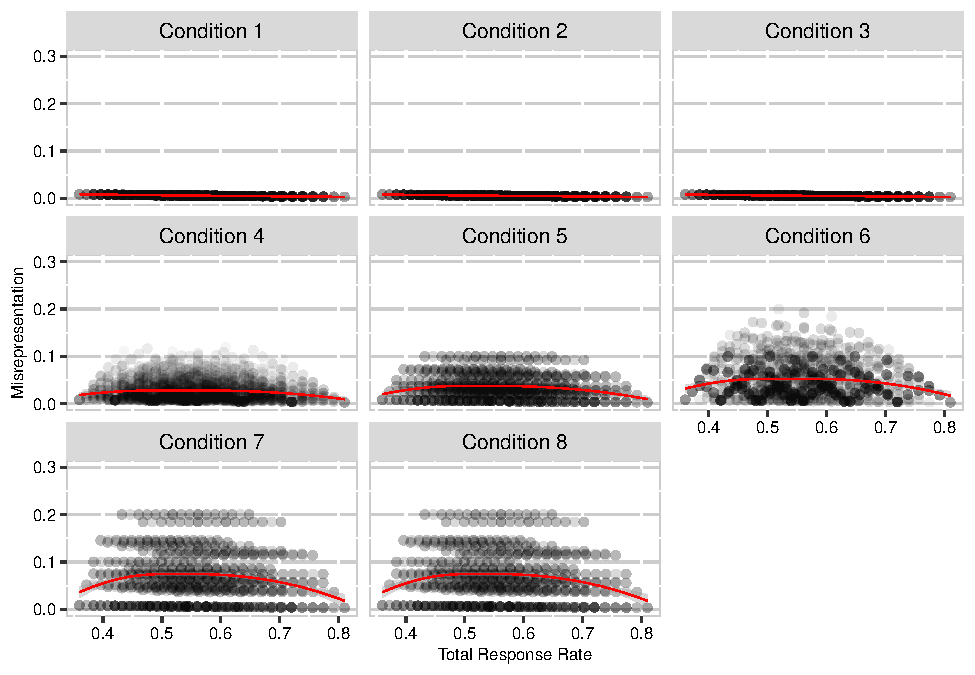
\includegraphics{focused-problem-solving_files/figure-latex/ResponseRate1-1.pdf}
\caption{\label{fig:ResponseRate1}Relationship between total response rate and misrepresentation.}
\end{figure}

\begin{figure}
\centering
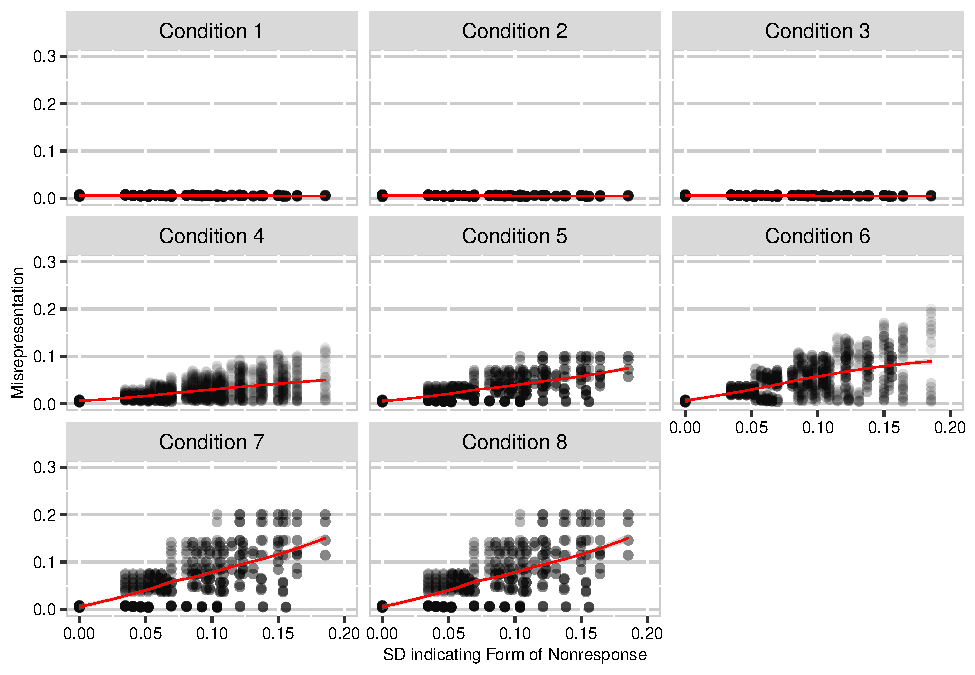
\includegraphics{focused-problem-solving_files/figure-latex/SDForm2-1.pdf}
\caption{\label{fig:SDForm2}Relationship between nonresponse form and misrepresentation.}
\end{figure}

\begin{figure}
\centering
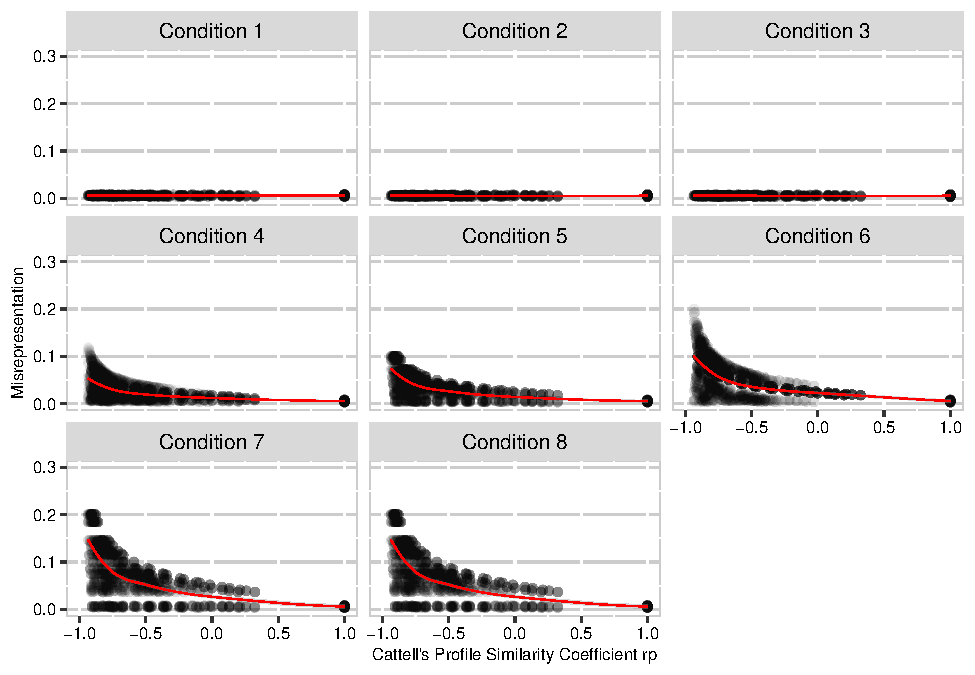
\includegraphics{focused-problem-solving_files/figure-latex/Cattell3-1.pdf}
\caption{\label{fig:Cattell3}Effect of subgroup sampling rate match with distributional form on population misrepresentation.}
\end{figure}

\begin{figure}
\centering
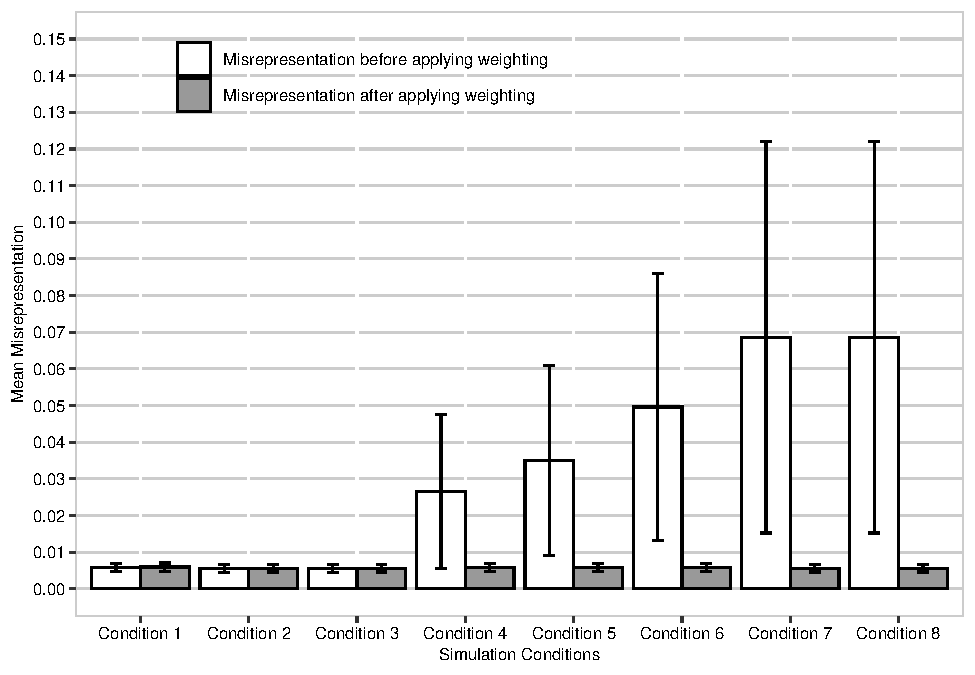
\includegraphics{focused-problem-solving_files/figure-latex/Overall4-1.pdf}
\caption{\label{fig:Overall4}Average absolute discrepancy (unweighted in white and weighted in grey) across the eight attitudinal conditions.}
\end{figure}

\subsection{Role of nonresponse form}\label{role-of-nonresponse-form}

\begin{figure}
\centering
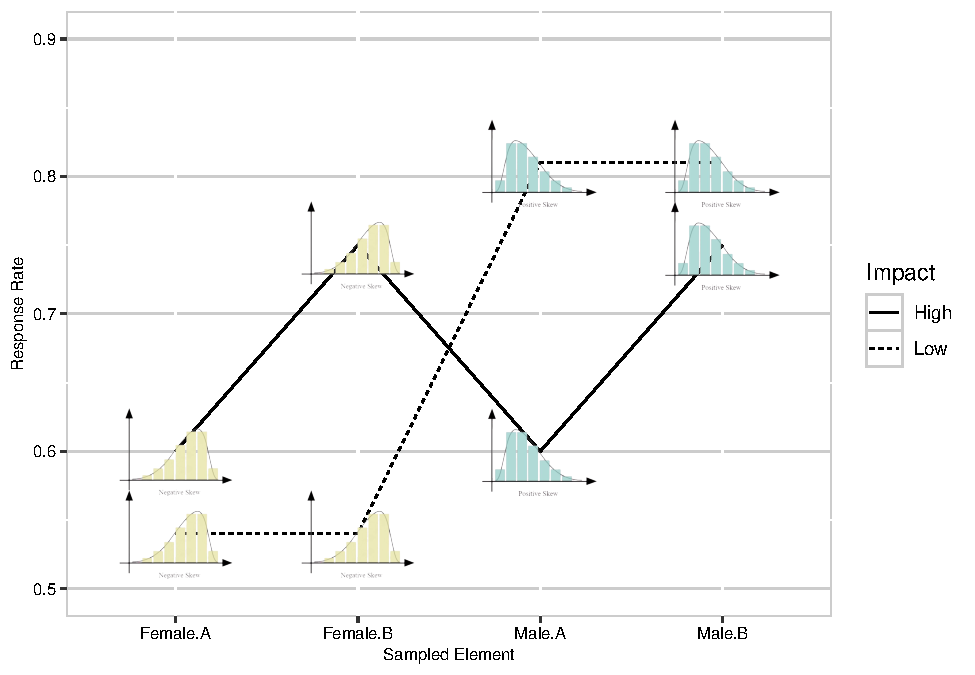
\includegraphics{focused-problem-solving_files/figure-latex/CattelExplain-1.pdf}
\caption{\label{fig:CattelExplain}Allocation of response rates relative to underlying distributional form and its impact on population misrepresentation (need to think through hi/lo given Dr Robinsons thoughts)}
\end{figure}

The systematic patterns of heteroskedasticity of the Figure \ref{fig:SDForm2} scatterplots should also be noted. There are \emph{active nonresponse} scenarios in which no error is present (see, for example, the lower right-hand portions of conditions 4 through 8 where discrepancy estimates of ``0'' persist at multiple points along the passive-active x-axis). These circumstances are simulated conditions within which the response rates ``parallel'' the \emph{population distributional form}. For example, in Condition Eight, the distributional forms across populations were: \(Positive Skew_{Male(A)}\), \(Positive Skew_{Male(B)}\), \(Negative Skew_{Female(A)}\), \(Negative Skew_{Female(B)}\). Response rates that ``mirror'' distributional patterns in extreme cases of active nonresponse (e.g., SD = .156; 54\%\textsubscript{Male(A)}, 54\%\textsubscript{Male(B)}, 81\%\textsubscript{Female(A)}, 81\%\textsubscript{Female(B)}) result in effectively zero error in the population mean approximation (average discrepancy = 0.00, \emph{SD} = 0.00). Alternatively, when the response rates are inverted for the SD=.156 cases, (e.g., 54\%\textsubscript{Male\_A}, 81\%\textsubscript{Male\_B}, 54\%\textsubscript{Female\_A}, 81\%\textsubscript{Female\_B}), there is substantial error in approximation (average discrepancy = 0.16, SD = 0.03). Here, it is not merely response rate or form that is associated with biased sample estimates, but rather the nature of response rate relative to existing attitudinal differences.\footnote{Don't think this is correct - maybe frame: ``sometimes the active non-response is non-troublesome - when it fully parallels the distributional proportions (?)'' \(\leftarrow\) still confusing. Looked at with Yang 3/1/24 and still confused - maybe leave in for reviewers to note and question.} See Figure \ref{fig:CattelExplain} for placeholder explanation.

To further expand upon this \emph{attitudinal form/pattern of nonresponse} interplay, the discrepancies between population constituency and sampling proportions were additionally evaluated through the lens of Cattell's profile similarity index (\(r_p\), Cattell, 1949; Cattell et al., 1966). \(r_p\) is sensitive to discrepancies in profile shape (pattern across profile components), elevation (average component score), and scatter (sum of individual components' deviation from the elevation estimate. Here, the profile similarity index references the relationship between the response rates (NEED YANG TO VERIFY - THINK THIS IS SSmale;SSfemale;SSdepta;SSdeptb from \texttt{combo} object) and sample sizes (cellrate.ma;cellrate.mb;cellrate.fa;cellrate.gb) across experimental \emph{cells}. For example, VERIFY BEFORE CLARIFYING HERE. Figure \ref{fig:Cattell3} demonstrates the pattern of unweighted sample mean deviation (from the population parameter) when this index is taken into consideration. Specifically, Figure \ref{fig:Cattell3} demonstrates a more pronounced \emph{form of} nonresponse association when underlying attitudinal distributions evidence group differences (e.g., incrementally across the 8 specified conditions), and in these scenarios, active nonresponse is shown to have a fairly large effect on error within the sample estimate (as well as systematically increasing degrees of heteroskedasticity paralleling the Cattell index; omnibus Breusch-Pagan {[}across conditions{]} = 3177.2, \emph{p} \textless{} .001). The curvilinear nature of these functions was estimated via hierarchical polynomial regression (excluding conditions 1, 2, and 3), with misrepresentation exhibiting a linear association across condition (\(R^2\) = 0.15, \emph{p} \textless{} .001) as well as incrementally across the Cattell index (\(\Delta{R^2}\) = 0.24, \emph{p} \textless{} .001), and also exhibiting an incremental polynomial effect (\(\Delta{R^2}\) = 0.07, \emph{p} \textless{} .001).

To further elaborate this point, consider, for example, Condition 4 as presented in Table \ref{tab:Tab1}. Here, three groups are characterized by similar distributions of attitudes (normally distributed) and one, Female.B, is characterized by negatively skewed attitudes. The greatest unweighted error here arises from sampling scenarios in which there are many Female.B (e.g., in our specifications, 6,400) and fewer males and Department A females\footnote{Because of the ``marginal'' versus ``cell'' specifications of population constituencies, our most extreme example here necessarily results in 400 Male.A's, 1,600 Male.B's, and 1,600 Female.A's. This was a decision based on keeping the population N's at 10,000 and certainly more extreme population constituency combinations could be examined in future like-minded explorations.}, but the female.b exhibit a much lower response rate (e.g., 20\%) than do other groups, who respond at a high rate (e.g., 80\%). That is, it is not merely response rate, but response rate within these identifiable groups, and whether or not those response rate differences parallel underlying attitudinal differences that drives sample misrepresentation.

\newpage

\section{References}\label{references}

\begingroup
\setlength{\parindent}{-0.5in}
\setlength{\leftskip}{0.5in}

\phantomsection\label{refs}
\begin{CSLReferences}{1}{0}
\bibitem[\citeproctext]{ref-R-papaja}
Aust, F., \& Barth, M. (2018). \emph{{papaja}: {Create} {APA} manuscripts with {R Markdown}}. \url{https://github.com/crsh/papaja}

\bibitem[\citeproctext]{ref-cattell_r_1949}
Cattell, R. B. (1949). R p and other coefficients of pattern similarity. \emph{Psychometrika}, \emph{14}(4), 279--298.

\bibitem[\citeproctext]{ref-cattell_taxonometric_1966}
Cattell, R. B., Coulter, M. A., \& Tsujioka, B. (1966). The taxonometric recognition of types and functional emergents. \emph{Handbook of Multivariate Experimental Psychology}, 288--329.

\bibitem[\citeproctext]{ref-mellahi_response_2016}
Mellahi, K., \& Harris, L. C. (2016). Response rates in business and management research: An overview of current practice and suggestions for future direction. \emph{British Journal of Management}, \emph{27}(2), 426--437.

\bibitem[\citeproctext]{ref-werner_reporting_2007}
Werner, S., Praxedes, M., \& Kim, H.-G. (2007). The reporting of nonresponse analyses in survey research. \emph{Organizational Research Methods}, \emph{10}(2), 287--295.

\end{CSLReferences}

\endgroup


\end{document}
